\scanpage{3}
\deleted{\unsure{Groupe fondamental}}

\uline{I}\quad Langage des schémas

\uline{II}\quad Étude élémentaire de \unsure{qqs} classes de morphismes

\uline{III}\quad Cohomologie des faisceaux cohérents.

\uline{IV}\quad Étude locale des morphismes

\uline{V}\quad Étude globale élémentaire des \deleted{quelques} morphismes.
\margin{[N.B. Y inclure propriétés de descente pour morph. \uline{étale}]} 

\uline{VI}\quad Procédés de construction.\deleted{\unsure{1}}

\uline{VII}\quad Schémas en groupes. fibrés principaux (\uline{définition} du \unsure{groupe fondamental})

\uline{VIII}\quad \deleted{Étude \unsure{des schémas} fibrés (\unsure{notions} \illegible{3} \unsure{faisceaux projectifs}; \illegible{3})}
\inserted{Picard et V.A.}

\deleted{\uline{\unsure{IX}}\quad Groupe fondamental}
\margin{$\longleftarrow$ pour la \unsure{coh.} étale\ldots}

\deleted{\uline{\unsure{X}}\quad \unsure{Schémas abéliens}}

\figure{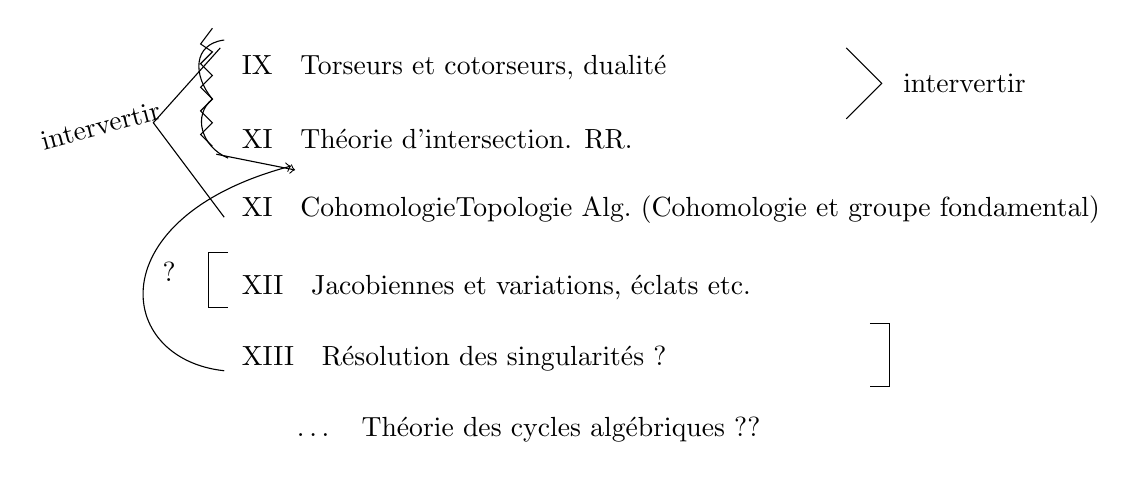
\begin{tikzpicture}[x=1cm,y=1cm]
\node[anchor=west] (ix) at (0,0) {\uline{IX}\quad Torseurs et cotorseurs, dualité};
\node[anchor=west] (x) at (0,-.9) {\uline{X}\deleted{\unsure{I}}\quad Théorie d'intersection. RR.};
\node[anchor=west,align=left] (xi) at (0,-1.8) {\uline{X\unsure{I}}\quad \deleted{\unsure{Cohomologie}}\inserted{\uline{Topologie Alg.}}\ (\deleted{Cohomologie et} groupe fondamental)};
\node[anchor=west] (xii) at (0,-2.8) {\uline{XII}\quad \unsure{Jacobiennes} \unsure{et variations}, \unsure{éclats} etc.};
\node[anchor=west] (xiii) at (0,-3.7) {\uline{XIII}\quad Résolution des singularités ?};
\node[anchor=west] at (.7,-4.6) {\unsure{\ldots}\quad Théorie des cycles \unsure{algébriques} ??};
\draw (-.1,.35) .. controls (-.5,.3) and (-.5,-.1) .. (-.25,-.4)
 .. controls (-.5,-.6) and (-.4,-1) .. (-.05,-1.15);
\draw (-.15,.25)--(-1,-.7)--(-.1,-1.9);
\node[anchor=east,rotate=15] at (-.8,-.5) {\unsure{intervertir}};
\draw[->] (-.2,-1.1)--(.8,-1.3);
\draw[->] (-.1,-3.85) .. controls (-1.5,-3.7) and (-1.7,-1.9) .. (.75,-1.25);
\node at (-.8,-2.6) {?};
\draw (-.05,-2.35)--(-.3,-2.35)--(-.3,-3.05)--(-.05,-3.05);
\draw (8.1,-3.25)--(8.35,-3.25)--(8.35,-4.05)--(8.1,-4.05);
\draw (7.8,.25)--(8.25,-.2)--(7.8,-.65);
\node[anchor=west] at (8.4,-.2) {\unsure{intervertir}};
\draw (-.25,.5)--(-.4,.3)--(-.25,.2)--(-.4,.05)--(-.25,-.1)--(-.4,-.25)--(-.25,-.4)--(-.4,-.55)--(-.25,-.7)--(-.4,-.85)--(-.25,-1);
\end{tikzpicture}}

\mspage{\unsure{2}}
